\chapter{Affine Algebra}

This chapter explores affine algebra, which is an extension of linear 
algebra that includes translations. Translations enable us to navigate 
affine subspaces, which are produced from affine bases. An affine 
subspace is basically a translated linear subspace, so affine 
subspaces can be geometrically interpreted as points, lines, 
planes, and hyperplanes with a local origin which do not necessarily 
coincide the standard origin.

\paragraph{Affine bases}

The fundamental object of an affine subspace is its affine basis.
An affine basis is a point and a set of zero or more vectors 
protruding from it. The point behaves as the origin, and the vectors 
are used to traverse the affine subspace which exists through their 
origin and is spanned by the \textit{independent} vectors.

\paragraph{Affine simplices}

Every unique \(n\)-dimensional affine basis has exactly one
corresponding \(n\)-dimensional affine simplex. An affine simplex
is a point, or a line segment, or a triangle, or a tetrahedron, 
or any of their higher dimensional analogues. Curved mathematical
objects are understood by tessellating them into affine simplices.
By understanding the affine algebra of simplices, we can better 
understand curved objects.

\paragraph{Affine subspaces}

By going the other way and expressing a simplex as a basis, we can 
navigate spaces spanned by simplices using vector addition and 
scalar multiplication. We could even, for instance, take the intersection 
of a space formed by one simplex with a space formed by another simplex.
Zooming out, we can imagine how this would be useful for understanding 
tessellated objects, which are composed of many simplices. 

\section{Affine algebra in \texorpdfstring{\(\mathbb{R}^{1}\)}{R1}}

We will begin our study of affine algebra with parametric objects
in \(\mathbb{R}^{1}\). This is because in order to illustrate 
affine transformations in higher dimensions, we will need to 
visualize an extra dimension. By starting in \(\mathbb{R}^{1}\), we 
can do affine transformations entirely in two dimensions, which we can
visualize easily.

\subsection{Parametric objects in \texorpdfstring{\(\mathbb{R}^{1}\)}{R1}}

There are exactly two classes of parametric objects which may exist in 
\(\mathbb{R}^{1}\): 
\begin{itemize}
    \item those which are tessellated by line segments, and  
    \item those which are tessellated by an individual point. 
\end{itemize}
This is no coincidence, since these are all the simplices whose bases 
have maximum dimension one. In general, the maximum dimensional possible 
simplex in a space is equal to the dimension of the space itself.

For example, a parametric line segment---a curve in 
\(\mathbb{R}^{1}\)---is tessellated by line segments, 
and a parametric point is tessellated by an individual point. Points 
and line segments are collectively referred to as the 
\textbf{0--1-dimensional simplices}. In general, an \(n\)-simplex is a 
set of \(n+1\) points, such that their basis representation is 
affine independent---which is analogous to linear independence.

This might all seem a bit abstract, so let's look at a couple parametric 
objects in \(\mathbb{R}^1\); remember, there are two types.
All line segments in \(\mathbb{R}^{1}\) are 1-dimensional parametric 
objects. All points in \(\mathbb{R}^{1}\) are 0-dimensional parametric 
objects. In order to obtain a tessellation, we take a sequence of samples
along the object, and connect the samples with simplices. For a
line segment, these simplices would be line segments; for a point, it would
be just the point itself. See Figure~\ref{fig:affine-R1tessellation} for 
the visual analogue.

\begin{figure}
    \centering
    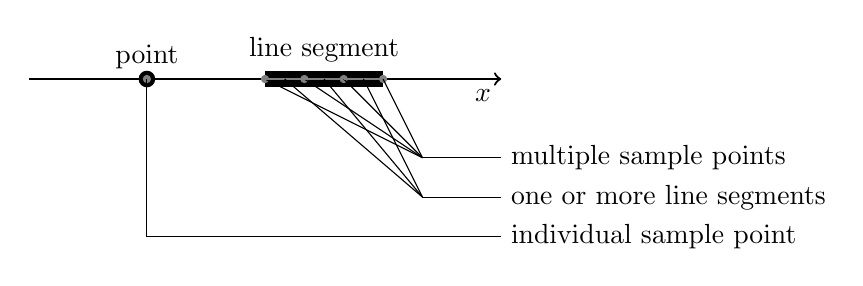
\begin{tikzpicture}
        \draw[thick,->] (-1,0) -- (5,0) node[below left] {\(x\)};
        \fill (0.5,0) circle[radius = 3pt] node[above] {point};
        \fill[gray] (0.5,0) circle[radius = 1.5pt];
        \draw[] (0.5,0) -- (0.5,-2) -- (5,-2) node[right] {individual sample point};
        \draw[line width = 6pt] (2,0) -- (3.5,0) node[above,pos=0.5]{line segment};
        \foreach[count = \c from 1] \x in {2,2.5,...,3.5} {
            \fill[gray] (\x,0) circle[radius = 1.5pt];
            \draw[] (\x,0) -- (4,-1);
            \ifnum\c=4\else\draw[thick,gray] (\x,0) -- ++(0.5,0);\fi
        }
        \draw[](4,-1) -- (5,-1) node[right] {multiple sample points};

        \foreach \x in {2.25,2.75,...,3.25} {
            \draw[] (\x,0) -- (4,-1.5);
        }
        \draw[](4,-1.5) -- (5,-1.5) node[right] {one or more line segments};
    \end{tikzpicture}
    \caption{Tessellated parametric objects in \(\mathbb{R}^{1}\).}
    \label{fig:affine-R1tessellation}
\end{figure}

\begin{example}
    Illustrate the tessellation of the parametric object defined by
    \[
        f(u) = 1+u,\ u\in[0,2],
    \]
    using five sample points in an arithmetic sequence.
\end{example}
\begin{solution}
    Every parametric object, in every dimension, is defined by two 
    components. The first component is the parametric equation, 
    and the second component is the domain. In this case, the 
    parametric equation is \(f(u) = 1+u\), and the domain is \([0,2]\). 

    A tessellated parametric object is a parametric object which is 
    approximated by simplices. To obtain a tessellation by an 
    arithmetic sequence, We find the start point \(a\), the stop point \(b\),
    and using the number of samples \(c\), the step size \[
        d = \frac{b-a}{c-1}.
    \]

    With all this information, we can draw a number line containing 
    both endpoints, and then place the sample points along it, starting 
    from the start point and incrementing by the step size until we reach the
    stop point. Finally, we connect the sample points with line segments.

    In this case, the start point is \(f(0) = 1\), the stop point is
    \(f(2) = 3\), and the step size is \((3-1)/(5-1) = 0.5\).
\end{solution}
\begin{remark}
    General methods for tessellating parametric objects become more
    advanced beyond \(\mathbb{R}^{1}\). We will briefly discuss some
    of these in \(\mathbb{R}^{2}\).
\end{remark}
Now we will discuss each of the simplicial classes.

\subsubsection{Points}

The matrix representation of a point simplex \(a\) in \(\mathbb{R}^{1}\) is 
\[
    \begin{bmatrix}
        a 
    \end{bmatrix}.
\]
The matrix simply contains the point's coordinate as its only element.
The affine basis representation of a point simplex is the same as its
matrix representation. This is because the dimension of a point is zero,
hence there being no protruding vectors in its basis---there's no space 
to span. See Figure~\ref{fig:affine-R1point} for the visual analogue.

\begin{figure}
    \centering 
    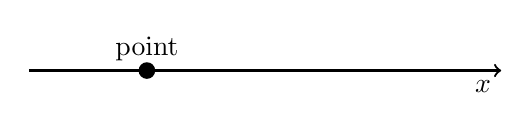
\begin{tikzpicture}
        \draw[thick,->] (-1,0) -- (5,0) node[below left] {\(x\)};
        \fill (0.5,0) circle[radius = 3pt] node[above] {point};
    \end{tikzpicture}
    \caption{A point simplex in \(\mathbb{R}^{1}\).}
    \label{fig:affine-R1point}
\end{figure}

\subsubsection{Line segments}

The matrix representation of a line segment simplex \(\{a,b\}\) in 
\(\mathbb{R}^{1}\) is represented by a \(2\times1\) matrix. 
The elements of this matrix are simply the coordinates of the 
two endpoints. 

To obtain the affine basis representation of this line segment matrix,
we replace the second row by its difference with the first---turning 
it into a difference vector---so that it can be added to the first 
to yield the original second point:
\[
    \underset{\mbox{simplex}}{
        \begin{bmatrix}
            a & b \\
        \end{bmatrix}
    }
    \sim
    \underset{\mbox{basis}}{
        \begin{bmatrix}
            a & b-a \\
        \end{bmatrix}
    }.
\]
Now, we have two equivalent representations of the same line segment.
See Figure~\ref{fig:affine-R1linesegment} for the visual analogue.
We usually start from a parametric object, and then inquire about its nature 
by tessellating it into simplices and using their affine basis representations.
We will explore this further in \(\mathbb{R}^{2}\) and \(\mathbb{R}^{3}\)
where the results become more interesting---involving solving systems of equations.
\begin{remark}
    A matrix is only a simplex representation if its basis 
    representation is affine independent; that is, if its protruding 
    vectors are linearly independent.
\end{remark}

\begin{figure}
    \centering 
    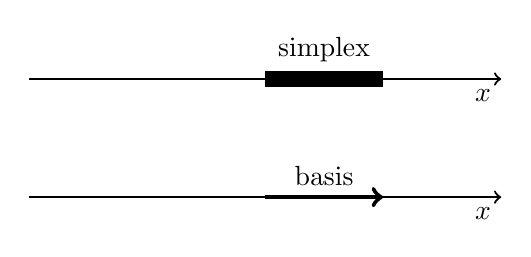
\begin{tikzpicture}
        \draw[thick,->] (-1,0) -- (5,0) node[below left] {\(x\)};
        \draw[line width = 6pt] (2,0) -- (3.5,0) node[above,pos=0.5]{simplex};

        \begin{scope}[yshift=-1.5cm]
            \draw[thick,->] (-1,0) -- (5,0) node[below left] {\(x\)};
            \draw[ultra thick,->] (2,0) -- (3.5,0) node[above,pos=0.5]{basis};
        \end{scope}
    \end{tikzpicture}
    \caption{The simplex and basis of a line segment in \(\mathbb{R}^{1}\).}
    \label{fig:affine-R1linesegment}
\end{figure}

\subsection{Linear transformations in \texorpdfstring{\(\mathbb{R}^{1}\)}{R1}}

A linear transformation in \(\mathbb{R}^{1}\) is simply a scaling
by some non-zero factor \(k\). This is because the only linear
transformation matrix which can exist in \(\mathbb{R}^{1}\) is a
\(1\times1\) matrix, which is simply a scalar. This has the effect of 
scaling the real line, including reflection and degeneration to a point.

Linear transformations can be thought of as a change of basis. Again,
change of basis might sound abstract, but it is really just 
taking one basis vector and changing it's displacement. 
Even more basically, take a nondegenerate vector from the origin, and 
make it's endpoint literally anything---even the origin, or even the 
original point in the case of the identity. Then, every other point 
in the line is scaled accordingly. 
See Figure~\ref{fig:affine-R1lineartransformation} for the visual analogue.

\begin{figure}
    \centering 
    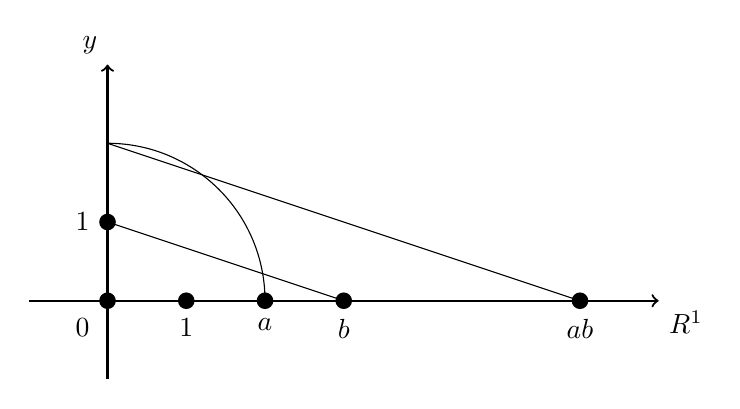
\begin{tikzpicture}
        \draw[thick,->] (-1,0) -- (7,0) node[below right] {\(\mathbb{R}^{1}\)};
        \draw[thick,->] (0,-1) -- (0,3) node[above left] {\(y\)};
        \fill (0,0) circle[radius = 3pt] node[below left=3pt] {\(0\)};
        \fill (1,0) circle[radius = 3pt] node[below=3pt] {\(1\)};
        \fill (0,1) circle[radius = 3pt] node[left=3pt] {\(1\)};
        \fill (2,0) circle[radius = 3pt] node[below=3pt] {\(a\)};
        \draw (2,0) arc[start angle=0,end angle=90,radius=2];
        \fill (3,0) circle[radius = 3pt] node[below=3pt] {\(b\)};
        \fill (6,0) circle[radius = 3pt] node[below=3pt] {\(ab\)};
        \draw (0,1) -- (3,0);
        \draw (0,2) -- (6,0);
    \end{tikzpicture}
    \caption{Scaling \(a\) by \(b\) in \(\mathbb{R}^{1}\).}
    \label{fig:affine-R1lineartransformation}
\end{figure}

\subsection{Affine transformations in \texorpdfstring{\(\mathbb{R}^{1}\)}{R1}}

Affine transformations are a strict superset of the linear
transformations, in that all linear transformations are affine
transformations even though not all affine transformations are
linear. In plain speak, affine transformations add translation
to our set of available transformations. This enables us to perform
transformations with respect to points which are not the origin.

These translations are enabled by orthogonally projecting our space---%
normally by one unit---into a new dimension. By doing this, we can
shear the extra dimension to move our origin. Finally, to obtain the
result of the transformation, we inverse orthogonally project our space
back onto the original region it occupied.

Alternatively, one can thing of affine transformations as a 
composition of a linear transformation and a translation.
First we perform the linear transformation, as in 
Figure~\ref{fig:affine-R1lineartransformation}, and then we 
perform the the translation, as in Figure~\ref{fig:affine-R1translation}. 
In particular, we project our space onto the line \(y=1\), shear the 
new dimension to move the origin, and then project back down to the \(x\)-axis.
Shearing is a linear transformation in that higher dimensional space, and 
we will soon study geometric linear transformation when we examine 
Figure~\ref{fig:affine-R2lineartransformation}.
\begin{remark}
    We are only concerned with the point \(t+ab\) when translating a point.
    If we translate a line segment \([a,c]\), then we obtain 
    the its affine image \([t+ab,t+cb]\). Each point would get its own 
    construction.
\end{remark}

\begin{figure}
    \centering
    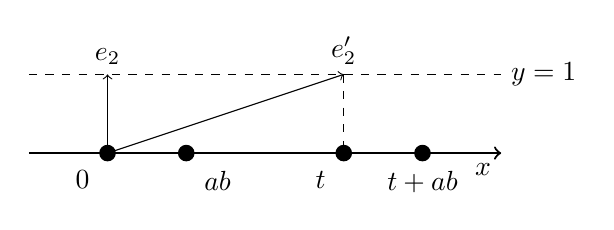
\begin{tikzpicture}
        \draw[thick,->] (-1,0) -- (5,0) node[below left] {\(x\)};
        \fill (0,0) circle[radius = 3pt] node[below left=3pt] {\(0\)};
        \fill (1,0) circle[radius = 3pt] node[below right=3pt] {\(ab\)};
        \fill (3,0) circle[radius = 3pt] node[below left=3pt] {\(t\)};
        \fill (4,0) circle[radius = 3pt] node[below=3pt] {\(t+ab\)};
        
        \draw[->] (0,0) -- (3,1) node[above]{\(e_2'\)};
        \draw[->] (0,0) -- (0,1) node[above]{\(e_2\)};
        \draw[dashed] (-1,1) -- (5,1) node[right]{\(y=1\)};
        \draw[dashed] (3,1) -- (3,0);
    \end{tikzpicture}
    \caption{Translating \([0,ab]\) by \(t\) in \(\mathbb{R}^{1}\).}
    \label{fig:affine-R1translation}
\end{figure}

Affine transformations in \(\mathbb{R}^{1}\) can be represented
by \(2\times2\) matrices of the form
\[
    \begin{bmatrix}
        k & t \\
        0 & 1
    \end{bmatrix},
\]
where \(k\) is the scaling factor, and \(t\) is the translation amount.
You might notice that a \(2\times2\) matrix cannot directly transform
a \(1\times1\) or a \(1\times2\) matrix. To resolve this, we augment 
the matrix by adding a second row with the value \(1\)---projecting  
into a new dimension:
\[
    \underset{\mbox{point}}{
        \begin{bmatrix}
            a \\
            1
        \end{bmatrix}
    }
    \qquad
    \underset{\mbox{line segment}}{
        \begin{bmatrix}
            a & b \\
            1 & 1
        \end{bmatrix}
    }.
\]
Now when we multiply the affine transformation matrix with the
augmented matrices, we obtain
\[
    \begin{bmatrix}
        k & t \\
        0 & 1
    \end{bmatrix}
    \begin{bmatrix}
        a \\
        1
    \end{bmatrix}
    =
    \begin{bmatrix}
        ka + t \\
        1
    \end{bmatrix}
\]
for points, and
\[
    \begin{bmatrix}
        k & t \\
        0 & 1
    \end{bmatrix}
    \begin{bmatrix}
        a & b \\
        1 & 1
    \end{bmatrix}
    =
    \begin{bmatrix}
        ka + t & kb + t \\
        1 & 1
    \end{bmatrix}
\]
for line segments. In both cases, we can discard the last row---%
projecting back down to \(\mathbb{R}^1\)---%
to obtain the transformed object in \(\mathbb{R}^{1}\).

\subsubsection{The inverse of an affine transformation}

The inverse of an affine transformation matrix is also an affine
transformation matrix. Not only that, but the inverse is computed in 
exactly the same way as with linear transformation matrices.

\subsection{Projective transformations in \texorpdfstring{\(\mathbb{R}^{1}\)}{R1}}

Projective transformations are a strict superset of affine
transformations, in that all affine transformations are projective
transformations even though not all projective transformations are
affine. In plain speak, projective transformations add perspective
to our set of available transformations. This enables us to perform
transformations which simulate the effect of viewing objects from
different vantage points.

Projective transformations are enabled by both altering the values the 
bottom row of the affine transformation matrix, and by modifying how we
multiply matrices---by adding an additional division step after the
multiplication step. Specifically, we divide each matrix component by 
the homogeneous component of its vector.
\begin{remark}
    We only perform the projective step when we are transforming 
    a parametric object---i.e., its tessellated simplices. We 
    \textbf{do not} perform the projective step when composing 
    multiple projective transformation matrices together.
\end{remark}

A projective transformation in \(\mathbb{R}^{1}\) can be represented
by \(2\times2\) matrices of the form
\[
    \begin{bmatrix}
        a & b \\
        c & d 
    \end{bmatrix},
\]
where \(c\) is not zero. When we multiply this matrix with the
augmented matrix of a line segment, we obtain
\[
    \begin{bmatrix}
        a & b \\
        c & d 
    \end{bmatrix}
    \begin{bmatrix}
        e & f \\
        1 & 1
    \end{bmatrix}
    =
    \begin{bmatrix}
        ae + b & af + b \\
        ce + d & cf + d
    \end{bmatrix}.
\]
by regular matrix multiplication. However, to complete the projective
transformation, we must divide each element in the first row by the
corresponding element in the second row:
\[
    \cdots=
    \begin{bmatrix}
        \frac{ae + b}{ce + d} & \frac{af + b}{cf + d} \\
        1 & 1
    \end{bmatrix}.
\]
Again, we can discard the last row to obtain the transformed object.

This all can seem very abstract, so let's analyze some what happens 
because of the \(c\) component. Notice that it scales the homogeneous 
component by the product of itself with the coordinate. This means that 
we are getting a scaling which is linearly dependent on the coordinate itself.
Of course, this means that the equation is linear---with a constant term.
When we divide by the homogeneous component afterward, we are 
effectively scaling the coordinate by the multiplicative inverse of a 
linear function. See Figure~\ref{fig:affine-R1projectivetransformation} 
for a visual analogue of transforming a line segment by a projective transformation.
\begin{remark}
    Functions of the form \[\frac{ax+b}{cx+d}\] are called 
    \textbf{Möbius transformations}. They are also called 
    \textbf{fractional linear transformations}, or the 
    \textbf{bilinear transformations}. We are essentially dealing 
    with real-valued Möbius transformations in this chapter.
\end{remark}

\begin{figure}
    \centering 
    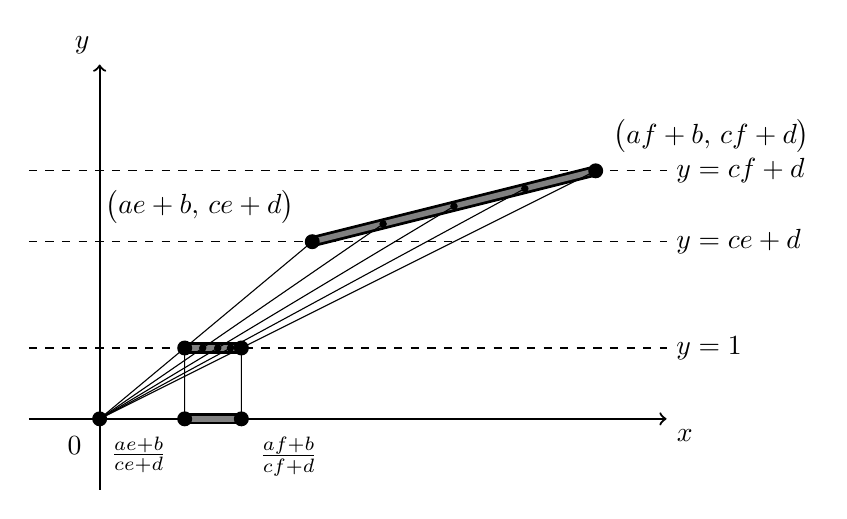
\begin{tikzpicture}[scale=0.9]
    
        % axes
        \draw[thick,->] (-1,0) -- (8,0) node[below right] {$x$};
        \draw[thick,->] (0,-1) -- (0,5) node[above left] {$y$};
    
        % y = 1 line
        \draw[dashed] (-1,1) -- (8,1) node[right] {$y=1$};
    
        % parameters: endpoints e,f
        \pgfmathsetmacro{\e}{2}
        \pgfmathsetmacro{\f}{4}
    
        % projective matrix parameters
        \pgfmathsetmacro{\a}{2}
        \pgfmathsetmacro{\b}{-1}
        \pgfmathsetmacro{\c}{0.5}
        \pgfmathsetmacro{\d}{1.5}
    
        % numerators and denominators
        \pgfmathsetmacro{\nE}{\a*\e + \b}
        \pgfmathsetmacro{\nF}{\a*\f + \b}
        \pgfmathsetmacro{\wE}{\c*\e + \d}
        \pgfmathsetmacro{\wF}{\c*\f + \d}
    
        % w-lines
        \draw[dashed] (-1,\wE) -- (8,\wE) node[right] {$y = ce + d$};
        \draw[dashed] (-1,\wF) -- (8,\wF) node[right] {$y = cf + d$};
    
        % origin
        \fill (0,0) circle (3pt) node[below left=3pt] {$0$};
    
        % endpoints in (numerator, denominator) space
        \coordinate (Eup) at (\nE,\wE);
        \coordinate (Fup) at (\nF,\wF);
    
        % segment in (ax+b, cx+d)
        \draw[
            preaction={draw=black,line width=4pt},
            postaction={draw=gray,line width=2pt}
        ] (Eup) -- (Fup);
    
        \fill (Eup) circle (3pt)
            node[above left=3pt] {$\bigl(ae+b,\,ce+d\bigr)$};
        \fill (Fup) circle (3pt)
            node[above right=3pt] {$\bigl(af+b,\,cf+d\bigr)$};
    
        % rays from origin
        \draw[thin] (0,0) -- (Eup);
        \draw[thin] (0,0) -- (Fup);
    
        % projected endpoints on y=1
        \coordinate (Elo) at ({\nE/\wE},1);
        \coordinate (Flo) at ({\nF/\wF},1);
    
        \draw[
            preaction={draw=black,line width=4pt},
            postaction={draw=gray,line width=2pt}
        ] (Elo) -- (Flo);
    
        \fill (Elo) circle (3pt);
        \fill (Flo) circle (3pt);
    
        % interior sample points along [e,f]
        \foreach \x in {0.25,0.5,0.75} {
            \pgfmathsetmacro{\X}{\e + \x*(\f-\e)}
            \pgfmathsetmacro{\nX}{\a*\X + \b}
            \pgfmathsetmacro{\wX}{\c*\X + \d}
    
            \coordinate (U) at (\nX,\wX);
            \coordinate (V) at ({\nX/\wX},1);
    
            \fill (U) circle (1.5pt);
            \fill (V) circle (1.5pt);
            \draw[thin] (0,0) -- (U);
        }
    
        % orthogonal projection to x-axis
        \draw[thin] (Elo) -- ({\nE/\wE},0)
            node[below left=3pt] {$\frac{ae+b}{ce+d}$};
        \draw[thin] (Flo) -- ({\nF/\wF},0)
            node[below right=3pt] {$\frac{af+b}{cf+d}$};
    
        \draw[
            preaction={draw=black,line width=4pt},
            postaction={draw=gray,line width=2pt}
        ] ({\nE/\wE},0) -- ({(\nF/\wF)},0);
    
        \fill ({\nE/\wE},0) circle (3pt);
        \fill ({\nF/\wF},0) circle (3pt);
    
    \end{tikzpicture}
    \caption{Projective transformation of a line segment in \(\mathbb{R}^{1}\).}
    \label{fig:affine-R1projectivetransformation}
\end{figure}

\subsubsection{The inverse of a projective transformation}

The inverse of a projective transformation matrix is also a projective
transformation matrix. Not only that, but the inverse is computed in 
exactly the same way as with affine and linear transformation matrices.
We just perform the homogeneous divide each pass.

% \subsection*{Exercises} % omitted for now

\section{Affine algebra in \texorpdfstring{\(\mathbb{R}^{2}\)}{R2}}

There are three classes of parametric objects which may exist in 
\(\mathbb{R}^{2}\): those which are tessellated by triangles, those 
which are tessellated by line segments, and those which are tessellated 
by individual points. This is no coincidence, since these are all the 
simplices whose affine bases have maximum dimension two.

A parametric curve is tessellated by line segments, and a parametric
surface is tessellated by triangles. A parametric point, of course,
is tessellated by an individual point. There can also be individual 
triangles, but they are non-parametric objects.

\subsection{Simplices in \texorpdfstring{\(\mathbb{R}^{2}\)}{R2}}

Points, line segments, and triangles are collectively referred to as the
\textbf{0--2-dimensional simplices}. In general, a simplex is a set of
one or more affine independent points. A set of points is affine independent if
the protruding vectors of their affine basis are linearly independent.

\subsubsection{Points}

A point simplex in \(\mathbb{R}^{2}\) is represented by a
1 \(2\times1\) matrix
\[
    \begin{bmatrix}
        a \\
        b 
    \end{bmatrix}.
\]
The matrix representation of a point simplex is the same as its affine
basis representation. 

\subsubsection{Line segments}

A line segment simplex in \(\mathbb{R}^{2}\) is represented by a 
\(2\times2\) matrix. To obtain the affine basis representation of this 
line segment, we replace the second column by its difference with the 
first---turning it into a difference vector---so that it can be added 
to the first to yield the original second point:
\[
    \underset{\mbox{simplex}}{
        \begin{bmatrix}
            a & c \\
            b & d
        \end{bmatrix}
    }
    \sim 
    \underset{\mbox{basis}}{
        \begin{bmatrix}
            a & c - a \\
            b & d - b
        \end{bmatrix}
    }.
\] 

\subsubsection{Triangles}

In the same way, a triangle simplex in 
\(\mathbb{R}^{2}\) is represented by a \(2\times3\) matrix.
To obtain the affine basis representation of this triangle,
we replace the second and third rows by their differences with 
the first---turning them into difference vectors:
\[
    \underset{\mbox{simplex}}{
        \begin{bmatrix}
            a & c & e \\
            b & d & f \\
        \end{bmatrix}
    }
    \sim
    \underset{\mbox{basis}}{
        \begin{bmatrix}
            a & c - a & e - a \\
            b & d - b & f - b \\
        \end{bmatrix}
    }.
\] 
See Figure~\ref{fig:affine-R2triangle} for the visual analogue of the simplex and basis of a triangle in \(\mathbb{R}^{2}\).
The lower dimensional analogues are found the same way.

\begin{figure}
    \centering
    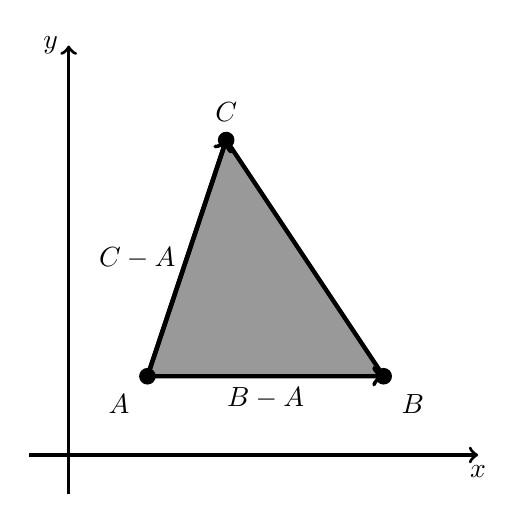
\begin{tikzpicture}
        \draw[very thick,->] (-0.5,0) -- (5.2,0) node[below] {$x$};
        \draw[very thick,->] (0,-0.5) -- (0,5.2) node[left] {$y$};
        \coordinate (A) at (1,1);
        \coordinate (B) at (4,1);
        \coordinate (C) at (2,4);
    
        \fill[gray!80] (A) -- (B) -- (C) -- cycle;
        \draw[ultra thick] (A) -- (B) -- (C) -- cycle;
    
        \fill (A) circle (3pt) node[below left=3pt] {$A$};
        \fill (B) circle (3pt) node[below right=3pt] {$B$};
        \fill (C) circle (3pt) node[above=3pt] {$C$};
    
        \draw[ultra thick,->] (A) -- (B)
            node[midway,below] {$B-A$};
        \draw[ultra thick,->] (A) -- (C)
            node[midway,left] {$C-A$};
    \end{tikzpicture}
    \caption{The simplex and basis of a triangle in \(\mathbb{R}^{2}\).}
    \label{fig:affine-R2triangle}
\end{figure}

\subsection{Parametric objects in \texorpdfstring{\(\mathbb{R}^{2}\)}{R2}}

Parametric objects in \(\mathbb{R}^{2}\) are tessellated by simplices.
Tessellated parametric objects are created by taking a domain space, 
sampling it, and tiling between the sample points with simplices.
Logistical sampling and tessellation of parametric objects is 
advanced. We focus on the case where an arithmetic sequence of samples 
is taken along each dimension.

\subsubsection{Parametric curves}

A parametric curve in \(\mathbb{R}^{2}\) is defined by an ordered 
list of two parametric equations, which both accept one parameter---on 
a common domain. For example, a circle is commonly defined by the 
parametric equation 
\[
    f\lparen u\rparen=
    \begin{bmatrix}
        \cos\lparen u\rparen \\
        \sin\lparen u\rparen
    \end{bmatrix},\ u\in\lbrack0,\tau\rbrack.
\]
If we traverse this parametric equation in even amounts---%
an arithmetic sequence along the domain, we will obtain a 
regular polygon which is composed of line segments. 
The number of line segments comprising the regular polygon---which 
approximate the circle---is one less than the number of samples.
See Figure~\ref{fig:affine-R2parametriccurves} for the visual analogue 
of parametric curves with different sample counts.

\begin{figure}
    \centering
    \foreach \samples in {5,7,20} {
    \begin{tikzpicture}
        \useasboundingbox (-1.5,-2) (1.5,1.5);
        \foreach \i in {0,...,\samples} {
            \pgfmathsetmacro{\angle}{\i*360/(\samples-1)}
            \fill ({cos(\angle)},{sin(\angle)}) circle (3pt);
            \draw ({cos(\angle)},{sin(\angle)}) -- ({cos(\angle+360/(\samples-1))},{sin(\angle+360/(\samples-1))});
        }
        \node at (0,-1.75) {samples: \samples};
    \end{tikzpicture}}
    
    \foreach \samples in {5,7,20} {
    \begin{tikzpicture}
        \useasboundingbox (-1.5,-2) (1.5,1.5);
        \foreach \i in {0,...,\samples} {
            \pgfmathsetmacro{\angle}{(\i-floor(\samples/2))*2*pi/(\samples-1)}
            \pgfmathparse{\i==\samples}
            \fill ({\angle/5},{sin(\angle r)}) circle (3pt);
            \ifnum\pgfmathresult=0
            \draw ({\angle/5},{sin(\angle r)}) -- ({(\angle+2*pi/(\samples-1))/5},{sin((\angle+2*pi/(\samples-1)) r)});
            \fi
        }
        \node at (0,-1.75) {samples: \samples};
    \end{tikzpicture}}
    \caption{Parametric curves in \(\mathbb{R}^{2}\) with different sample counts.}
    \label{fig:affine-R2parametriccurves}
\end{figure}

More generally, we have a formula of the form 
\begin{equation}
    f\lparen u\rparen=
    \begin{bmatrix}
        g\lparen u\rparen \\
        h\lparen u\rparen
    \end{bmatrix},\ u\in{}D,
\end{equation}
where \(D\) is a continuous finite subset of \(\mathbb{R}\).

\subsubsection{Parametric surfaces}

A parametric surface in \(\mathbb{R}^{2}\) is defined by an ordered 
list of two parameric equations, which both accept two parameters---on 
a common domain. For example, a disk is commonly defined by the 
parametric equation 
\[
    f\lparen u,v\rparen=
    \begin{bmatrix}
        v\cos\lparen u\rparen \\
        v\sin\lparen u\rparen
    \end{bmatrix},\ u\in\lbrack0,\tau\rbrack,\ v\in\lbrack0,1\rbrack.
\]
If we traverse this parametric equation in even amounts---%
an arithmetic sequence along each dimension of the domain, we will 
obtain a filled regular polygon composed of triangles. 
The number of triangles 
comprising the filled regular polygon---which approximates the disk---is 
one less than the number of \(u\) samples---\(u_s\)---multiplied by 
one less than the number of \(v\) samples---\(v_s\), all multiplied by 
two---because there are two triangles for every small rectangle on the 
domain. Of course, in the case of triangulation, there may be 
degenerate triangles, so the actual number of triangles is the 
theoretical number, minus the number of degenerate triangles.
See Figure~\ref{fig:affine-R2projectivetransformation} for the visual analogue of
parametric surfaces with different sample counts.

\begin{figure}
    \centering
    \foreach \usamples in {5,7} {
    \foreach \vsamples in {3,6,10} {
    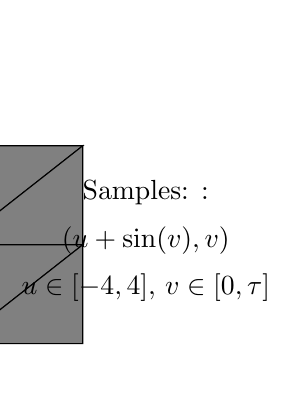
\begin{tikzpicture}[scale=0.2]
        \useasboundingbox[scale=1.5] (-5,-10) rectangle (5,5);
        \pgfmathsetmacro{\ustart}{-4}
        \pgfmathsetmacro{\ustop}{4}
        % \pgfmathsetmacro{\usamples}{7}
        \pgfmathsetmacro{\ustep}{(\ustop-\ustart)/(\usamples-1)}
        \pgfmathsetmacro{\vstart}{0}
        \pgfmathsetmacro{\vstop}{2*pi}
        % \pgfmathsetmacro{\vsamples}{12}
        \pgfmathsetmacro{\vstep}{(\vstop-\vstart)/(\vsamples-1)}
        \foreach \u[parse=true] in {\ustart,\ustart+\ustep,...,\ustop} {
            \foreach \v[parse=true] in {\vstart,\vstart+\vstep,...,\vstop} {
                \filldraw[fill=gray] 
                    ({\u+sin(\v r)},\v) --
                    ({\u+\ustep+sin((\v+\vstep) r)},{\v+\vstep}) --
                    ({\u+\ustep+sin(\v r)},{\v}) --
                    cycle
                ;
                \filldraw[fill=gray] 
                    ({\u+sin(\v r)},\v) --
                    ({\u+\ustep+sin((\v+\vstep) r)},{\v+\vstep}) --
                    ({\u+sin((\v+\vstep) r)},{\v+\vstep}) --
                    cycle
                ;
            }
        }
        \node at (0,-3) {Samples: \usamples:\vsamples};
        \node at (0,-6) {\((u+\sin(v),v)\)};
        \node at (0,-9) {\(u\in[-4,4],\,v\in[0,\tau]\)};
    \end{tikzpicture}}\par}
    \foreach \usamples in {3,7} {
    \foreach \vsamples in {4,7,10} {
    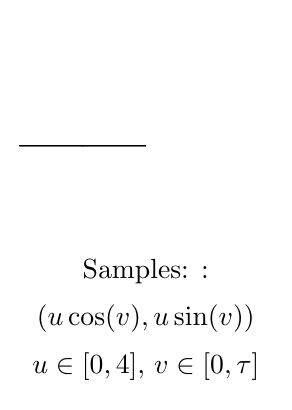
\begin{tikzpicture}[scale=0.2]
        \useasboundingbox[scale=1.5] (-5,-10) rectangle (5,5);
        \pgfmathsetmacro{\ustart}{0}
        \pgfmathsetmacro{\ustop}{4}
        % \pgfmathsetmacro{\usamples}{7}
        \pgfmathsetmacro{\ustep}{(\ustop-\ustart)/(\usamples-1)}
        \pgfmathsetmacro{\vstart}{0}
        \pgfmathsetmacro{\vstop}{2*pi}
        % \pgfmathsetmacro{\vsamples}{12}
        \pgfmathsetmacro{\vstep}{(\vstop-\vstart)/(\vsamples-1)}
        \foreach \u[parse=true] in {\ustart,\ustart+\ustep,...,\ustop} {
            \foreach \v[parse=true] in {\vstart,\vstart+\vstep,...,\vstop} {
                \filldraw[fill=gray] 
                    ({\u*cos(\v r)},{\u*sin(\v r)}) --
                    ({(\u+\ustep)*cos((\v+\vstep) r)},{(\u+\ustep)*sin((\v+\vstep) r)}) --
                    ({(\u+\ustep)*cos(\v r)},{{(\u+\ustep)*sin(\v r)}}) --
                    cycle
                ;
                \filldraw[fill=gray] 
                    ({\u*cos(\v r)},{\u*sin(\v r)}) --
                    ({(\u+\ustep)*cos((\v+\vstep) r)},{(\u+\ustep)*sin((\v+\vstep) r)}) --
                    ({\u*cos((\v+\vstep) r)},{{\u*sin((\v+\vstep) r)}}) --
                    cycle
                ;
            }
        }
        \node at (0,-8) {Samples: \usamples:\vsamples};
        \node at (0,-11) {\((u\cos(v),u\sin(v))\)};
        \node at (0,-14) {\(u\in[0,4],\,v\in[0,\tau]\)};
    \end{tikzpicture}}\par}
    \caption{Parametric surfaces in \(\mathbb{R}^{2}\) with different sample counts.}
\end{figure}

More generally, we have a formula of the form 
\begin{equation}
    f\lparen u,v\rparen=
    \begin{bmatrix}
        g\lparen u,v\rparen \\
        h\lparen u,v\rparen
    \end{bmatrix},\ u\in D_{1},\ v\in D_{2}
\end{equation}
where \(D_{1},D_{2}\) are continuous finite subsets of \(\mathbb{R}\).

\subsubsection{Parametric points}

A parametric point in \(\mathbb{R}^{2}\) is defined by an ordered 
list of two parameric equations, which both accept zero parameters; 
they just output constants. For example, a point centered at 
\(\lparen1,2\rparen\) is defined by the parametric equation 
\[
    f=
    \begin{bmatrix}
        1 \\
        2
    \end{bmatrix}.
\]
The general parameterization of a point is 
\begin{equation}
    f=
    \begin{bmatrix}
        g \\
        h
    \end{bmatrix},
\end{equation}
where \(g,h\) have no dependencies.

\subsection{Linear transformations in \texorpdfstring{\(\mathbb{R}^{2}\)}{R2}}

In general, a linear transformation is a change of linear basis vectors.
Nondegenerate transformations have the property that they transform 
simplices into simplices.

\subsubsection{Linear transformations on simplices}

Suppose we have a tile---for instance, a triangle---which is represented by some matrix
\[
    \begin{bmatrix}
        a & b \\
        c & d \\
        e & f
    \end{bmatrix},
\]
and we wanted to transform it by a \(2\times2\) linear transformation matrix 
\[
    \begin{bmatrix}
        g & h \\
        i & j
    \end{bmatrix}.
\]
This would yield the product
\[
    \begin{bmatrix}
        a & b \\
        c & d \\
        e & f
    \end{bmatrix}
    \begin{bmatrix}
        g & h \\
        i & j
    \end{bmatrix}
    =
    \begin{bmatrix}
        ag+bi & ah+bj \\
        cg+di & ch+dj \\
        eg+fi & eh+fj
    \end{bmatrix}.
\]
This product retains the property of being a triangle in the plane, 
unless the transformation has determinant zero, which would be a 
projection onto a lower-dimensional subspace.

Let's analyze the effect of a linear transformation on a point.
The point is represented by a \(2\times1\) matrix
\[
    \begin{bmatrix}
        a \\
        b 
    \end{bmatrix},
\]
and the linear transformation is represented by a \(2\times2\) matrix
\[
    \begin{bmatrix}
        g & h \\
        i & j
    \end{bmatrix}.
\]
The product of these two matrices is
\[
    \begin{bmatrix}
        a \\
        b 
    \end{bmatrix}
    \begin{bmatrix}
        g & h \\
        i & j
    \end{bmatrix}
    =
    \begin{bmatrix}
        ag+bi \\
        ah+bj
    \end{bmatrix}.
\]
See Figure~\ref{fig:affine-R2lineartransformation} for the visual 
analogue of a linear transformation of a point in \(\mathbb{R}^{2}\).

\begin{figure}
    \centering
    \pgfmathsetmacro{\azimuth}{110}
    \pgfmathsetmacro{\elevation}{30}
    \pgfmathsetmacro{\longitude}{60}
    \pgfmathsetmacro{\latitude}{30}
    \tdplotsetmaincoords{90-\elevation}{\azimuth}
    \begin{tikzpicture}[tdplot_main_coords,very thin,scale=0.7,font=\scriptsize]
        \draw[->] (-5,0) -- (5,0) node[pos=1.1]{\(x\)};
        \draw[->] (0,-5) -- (0,5) node[pos=1.1]{\(y\)};
        \draw[->] (0,0,-5) -- (0,0,5) node[pos=1.1]{\(z\)};
        \begin{scope}
            % clip and blank out sphere
            \clip[
                tdplot_screen_coords
                ,postaction = {
                    %tdplot_screen_coords
                    ,fill
                    ,white
                }
            ] (0,0) circle [radius = {1}];
            \draw[densely dashed] 
                (-2.5,0,0) -- (1,0,0);
            \draw[densely dashed] 
                (0,-1.5,0) -- (0,1,0);
            \draw[densely dashed] 
                (0,0,-1.5) -- (0,0,1);
            \draw[tdplot_screen_coords]
                (0,0) circle [radius = {1}];
            \draw[densely dashed]
                (\azimuth:1) arc [
                    start angle = {\azimuth}
                    ,end angle = {\azimuth+180}
                    ,radius = {1}
                ];
            \draw (\azimuth:1) arc [
                    start angle = {\azimuth}
                    ,end angle = {\azimuth-180}
                    ,radius = {1}
                ];
                \coordinate (O) at (0,0);
                \coordinate (N) at (0,0,1);
                \draw 
                    (N) -- (0,0,1.5)
                    (1,0,0) -- (2.5,0,0)
                    (0,1,0) -- (0,1.5,0)
                    ;
        \end{scope}
        \pgfmathsetmacro{\pointradius}{0.05}
        \begin{scope}[tdplot_screen_coords]
            \fill 
                (O) circle[radius = \pointradius] 
                node[left]{$\scriptstyle O$};
            \fill 
                (N) circle[radius = \pointradius]
                node[left]{$\scriptstyle 1$};
        \end{scope}
        \pgfmathsetmacro{\a}{-1.5}
        \pgfmathsetmacro{\b}{2}
        \draw[->] (0,0) -- (\a,\b) node[pos=1.3]{\((a,b)\)};
        \pgfmathsetmacro{\c}{1}
        \pgfmathsetmacro{\d}{3}
        \draw[->] (0,0) -- (\c,\d) node[pos=1.3]{\((c,d)\)};
        \pgfmathsetmacro{\e}{2}
        \pgfmathsetmacro{\f}{-1}
        \draw[->] (0,0) -- (\e,\f) node[pos=1.3]{\((e,f)\)};
        \pgfmathsetmacro{\g}{\c*\a+\e*\b}
        \pgfmathsetmacro{\h}{\d*\a+\f*\b}
        \draw[->] (0,0) -- (\g,\h) node[pos=1.2]{\((g,h)\)};
        \pgfmathsetmacro{\A}{atan2(\b,0)}
        \draw[domain=0:pi/2] plot (
            {\b*sin(\x r)*cos(\A)},
            {\b*sin(\x r)*sin(\A)},
            {\b*cos(\x r)}
        );
        \pgfmathsetmacro{\A}{atan2(0,\a)}
        \draw[domain=0:pi/2] plot (
            {abs(\a)*sin(\x r)*cos(\A)},
            {abs(\a)*sin(\x r)*sin(\A)},
            {abs(\a)*cos(\x r)}
        );
        \draw[densely dotted]
            (\a,\b) -- (\a,0)
            (\a,\b) -- (0,\b)
            (\a*\c,\a*\d) -- (\g,\h)
            (\b*\e,\b*\f) -- (\g,\h)
        ;
        \draw 
            (0,0,1) -- (\c,\d)
            (0,0,{abs(\a)}) -- (\a*\c,\a*\d)
            (0,0) -- (\a*\c,\a*\d) node[above left]{$(ac,ad)$}
            (0,0,1) -- (\e,\f)
            (0,0,\b) -- (\b*\e,\b*\f)
            (0,0) -- (\b*\e,\b*\f) node[below left]{$(be,bf)$}
        ;
    \end{tikzpicture}
    \caption{A general linear transformation of a point in \(\mathbb{R}^{2}\).}
    \label{fig:affine-R2lineartransformation}
\end{figure}

\subsubsection{Elementary transformations}

The elementary transformations arise from the elementary row 
operations. All linear transformations can be constructed from
compositions of these elementary transformations.

The identity transformation is represented by the matrix
\[
    \begin{bmatrix}
        1 & 0 \\
        0 & 1
    \end{bmatrix}.
\]
There are three classes of elementary transformations:
\begin{enumerate}
    \item row scaling,
    \item row swapping, and
    \item addition of a row's scalar multiple to another row.
\end{enumerate}
This yields three types of elementary matrices:
\[
    \begin{bmatrix}
        k & 0 \\
        0 & 1
    \end{bmatrix},\quad
    \begin{bmatrix}
        0 & 1 \\
        1 & 0
    \end{bmatrix},\quad
    \begin{bmatrix}
        1 & m \\
        0 & 1
    \end{bmatrix}.
\]
These correspond to scaling along the \(x\)-axis, reflecting in the 
\(x\)-dimension, and shearing the \(x\)-axis, respectively.

\paragraph{Transformations as a change of basis}

A linear transformation is basically just a swap of basis vectors.
We can use vector-valued functions to define new bases. For 
example, the function 
\[
    f(u)=
    \begin{bmatrix}
        \cos(u) & \cos(u+\tau/4) \\
        \sin(u) & \sin(u+\tau/4)
    \end{bmatrix}
\]
defines a new basis for every value of \(u\), based on a 
parameterization---in this case, that of a circle. 
If we were to animate the effect of transforming a plane 
by this changing basis, we would see the plane rotating.
We could do this with any parametric curve which defines
two linearly independent vectors for every value of its parameter.

\subsection{Affine transformations in \texorpdfstring{\(\mathbb{R}^{2}\)}{R2}}

Just like in \(\mathbb{R}^{1}\), affine transformations in \(\mathbb{R}^{2}\)
are enabled by orthogonally projecting our space---normally by one unit---%
into a new dimension. By doing this, we can shear the extra dimension to
move our origin. Finally, to obtain the result of the transformation, we inverse 
orthogonally project our space back onto the original region it occupied.
If we take the vector \((g,h)\) from Figure~\ref{fig:affine-R2lineartransformation}, 
and we add a translation vector \((t_x,t_y)\) to it, we will have the 
effect of an affine transformation. For example, the affine transformation 
\[
\begin{bmatrix}
c & e & t_x \\
d & f & t_y \\
0 & 0 & 1
\end{bmatrix}
\begin{bmatrix}
a \\
b \\
1
\end{bmatrix}
=
\begin{bmatrix}
c a + e b + t_x \\
d a + f b + t_y \\
1
\end{bmatrix}
\]
is illustrated in Figure~\ref{fig:affine-R2affinetransformation}.
Just like in \(\mathbb{R}^{1}\), the affine transformation is a linear transformation
in an extra dimension in combination with a projection. We illustrated linear transformations in 
\(\mathbb{R}^{1}\) and \(\mathbb{R}^{2}\) by using similar triangles in an extra dimension, as in 
Figure~\ref{fig:affine-R2lineartransformation}. To illustrate a linear 
transformation in \(\mathbb{R}^{3}\), we would need a fourth dimension,
which is difficult to visualize. However, The intuition we have built up for linear transformations in \(\mathbb{R}^{1}\) and \(\mathbb{R}^{2}\)
is the same intuition we would use for linear transformations in \(\mathbb{R}^{3}\) and higher dimensions.

\begin{figure}
    \centering 
    \pgfmathsetmacro{\azimuth}{110}
    \pgfmathsetmacro{\elevation}{30}
    \pgfmathsetmacro{\longitude}{60}
    \pgfmathsetmacro{\latitude}{30}
    \tdplotsetmaincoords{90-\elevation}{\azimuth}
    \begin{tikzpicture}[tdplot_main_coords,very thin,scale=0.7,font=\scriptsize]
        \draw[->] (-5,0) -- (5,0) node[pos=1.1]{\(x\)};
        \draw[->] (0,-5) -- (0,5) node[pos=1.1]{\(y\)};
        \draw[->] (0,0,-5) -- (0,0,5) node[pos=1.1]{\(z\)};
        \begin{scope}
            % clip and blank out sphere
            \clip[
                tdplot_screen_coords
                ,postaction = {
                    %tdplot_screen_coords
                    ,fill
                    ,white
                }
            ] (0,0) circle [radius = {1}];
            \draw[densely dashed] 
                (-2.5,0,0) -- (1,0,0);
            \draw[densely dashed] 
                (0,-1.5,0) -- (0,1,0);
            \draw[densely dashed] 
                (0,0,-1.5) -- (0,0,1);
            \draw[tdplot_screen_coords]
                (0,0) circle [radius = {1}];
            \draw[densely dashed]
                (\azimuth:1) arc [
                    start angle = {\azimuth}
                    ,end angle = {\azimuth+180}
                    ,radius = {1}
                ];
            \draw (\azimuth:1) arc [
                    start angle = {\azimuth}
                    ,end angle = {\azimuth-180}
                    ,radius = {1}
                ];
                \coordinate (O) at (0,0);
                \coordinate (N) at (0,0,1);
                \draw 
                    (N) -- (0,0,1.5)
                    (1,0,0) -- (2.5,0,0)
                    (0,1,0) -- (0,1.5,0)
                    ;
        \end{scope}
        \pgfmathsetmacro{\pointradius}{0.05}
        \begin{scope}[tdplot_screen_coords]
            \fill 
                (O) circle[radius = \pointradius] 
                node[left]{$\scriptstyle O$};
            \fill 
                (N) circle[radius = \pointradius]
                node[left]{$\scriptstyle 1$};
        \end{scope}
        \pgfmathsetmacro{\a}{-1.5}
        \pgfmathsetmacro{\b}{2}
        \draw[->] (0,0) -- (\a,\b) node[pos=1.3]{\((a,b)\)};
        \pgfmathsetmacro{\c}{1}
        \pgfmathsetmacro{\d}{3}
        \draw[->] (0,0) -- (\c,\d) node[pos=1.3]{\((c,d)\)};
        \pgfmathsetmacro{\e}{2}
        \pgfmathsetmacro{\f}{-1}
        \draw[->] (0,0) -- (\e,\f) node[pos=1.3]{\((e,f)\)};
        \pgfmathsetmacro{\g}{\c*\a+\e*\b}
        \pgfmathsetmacro{\h}{\d*\a+\f*\b}
        \draw[->] (0,0) -- (\g,\h) node[pos=1.2]{\((g,h)\)};
        % \pgfmathsetmacro{\A}{atan2(\b,0)}
        % \draw[domain=0:pi/2] plot (
        %     {\b*sin(\x r)*cos(\A)},
        %     {\b*sin(\x r)*sin(\A)},
        %     {\b*cos(\x r)}
        % );
        % \pgfmathsetmacro{\A}{atan2(0,\a)}
        % \draw[domain=0:pi/2] plot (
        %     {abs(\a)*sin(\x r)*cos(\A)},
        %     {abs(\a)*sin(\x r)*sin(\A)},
        %     {abs(\a)*cos(\x r)}
        % );
        \draw[densely dotted]
            (\a,\b) -- (\a,0)
            (\a,\b) -- (0,\b)
            (\a*\c,\a*\d) -- (\g,\h)
            (\b*\e,\b*\f) -- (\g,\h)
        ;
        \draw 
            % (0,0,1) -- (\c,\d)
            % (0,0,{abs(\a)}) -- (\a*\c,\a*\d)
            (0,0) -- (\a*\c,\a*\d) node[above left]{$(ac,ad)$}
            % (0,0,1) -- (\e,\f)
            % (0,0,\b) -- (\b*\e,\b*\f)
            (0,0) -- (\b*\e,\b*\f) node[below left]{$(be,bf)$}
        ;
        \pgfmathsetmacro{\tx}{5}
        \pgfmathsetmacro{\ty}{4}
        \draw[green,->] (0,0) -- (\tx,\ty,1) node[right,]{\((t_x,t_y)\)};
        \draw[green,->,dashed] (0,0) -- (\tx,\ty);
        \draw[orange,->,dashed] (\tx,\ty,1) -- (\tx+\a*\c,\ty+\a*\d,1);
        \draw[orange,->,dashed] (\tx,\ty,1) -- (\tx+\b*\e,\ty+\b*\f,1);
        \draw[orange,->,dashed] (0,0,1) -- (\a*\c,\a*\d,1);
        \draw[orange,->,dashed] (0,0,1) -- (\b*\e,\b*\f,1);
        \draw[orange,->] (\tx,\ty) -- (\tx+\a*\c,\ty+\a*\d);
        \draw[orange,->] (\tx,\ty) -- (\tx+\b*\e,\ty+\b*\f);
        \draw[densely dotted]
            (\tx+\a*\c,\ty+\a*\d) -- (\tx+\g,\ty+\h)
            (\tx+\b*\e,\ty+\b*\f) -- (\tx+\g,\ty+\h)
        ;
        \draw[->,orange] (\tx,\ty) -- (\tx+\g,\ty+\h) node[pos=1.2]{\((g,h)'\)};
    \end{tikzpicture}
    \caption{The effect of an affine transformation on a point in \(\mathbb{R}^{2}\).}
    \label{fig:affine-R2affinetransformation}
\end{figure}

An affine transformation in \(\mathbb{R}^{2}\) can be represented
by \(3\times3\) matrices of the form
\[
    \begin{bmatrix}
        a & b & t_{x} \\
        c & d & t_{y} \\
        0 & 0 & 1
    \end{bmatrix},
\]
where the \(2\times2\) submatrix in the upper-left corner is a linear
transformation matrix, and \(t_{x},t_{y}\) are the translation amounts
along the \(x\) and \(y\) axes, respectively.

To apply this affine transformation matrix to a point, line segment,
or triangle, we augment the matrix of the simplex with an extra 
row of ones. For example, the affine transformation of a triangle 
can be expressed as
\[
    \begin{bmatrix}
        a & b & t_{x} \\
        c & d & t_{y} \\
        0 & 0 & 1
    \end{bmatrix}
    \begin{bmatrix}
        e & f & g \\
        h & i & j \\
        1 & 1 & 1
    \end{bmatrix}
    =
    \begin{bmatrix}
        ae+ch+t_{x} & af+ci+t_{x} & ag+cj+t_{x} \\
        be+dh+t_{y} & bf+di+t_{y} & bg+dj+t_{y} \\
        1 & 1 & 1
    \end{bmatrix}.
\]

\subsection{Projective transformations in \texorpdfstring{\(\mathbb{R}^{2}\)}{R2}}

Projective transformations in \(\mathbb{R}^{2}\) are enabled by both
altering the values the bottom row of the affine transformation matrix,
and by modifying how we multiply matrices---by adding an additional
division step after the multiplication step, as we did in \(\mathbb{R}^{1}\).

A projective transformation in \(\mathbb{R}^{2}\) can be represented
by \(3\times3\) matrices of the form
\[
    \begin{bmatrix}
        a & b & c \\
        d & e & f \\
        g & h & i 
    \end{bmatrix},
\]
where at least one of \(g,h\) is not zero. When we multiply this matrix
with the augmented matrix of a triangle, we obtain
\[
    \begin{bmatrix}
        a & b & c \\
        d & e & f \\
        g & h & i 
    \end{bmatrix}
    \begin{bmatrix}
        j & k & l \\
        m & n & o \\
        1 & 1 & 1
    \end{bmatrix}
    =
    \begin{bmatrix}
        aj+bm+c & ak+bn+c & al+bo+c \\
        dj+em+f & dk+en+f & dl+eo+f \\
        gj+hm+i & gk+hn+i & gl+ho+i
    \end{bmatrix}.
\]
However, to complete the projective transformation, we must divide
each element in the first and second rows by the corresponding element 
in the last row. The matrix then becomes
\[
    \cdots =
    \begin{bmatrix}
        \frac{aj+bm+c}{gj+hm+i} & \frac{ak+bn+c}{gk+hn+i} & \frac{al+bo+c}{gl+ho+i} \\
        \frac{dj+em+f}{gj+hm+i} & \frac{dk+en+f}{gk+hn+i} & \frac{dl+eo+f}{gl+ho+i} \\
        1 & 1 & 1
    \end{bmatrix}.
\]
Figure~\ref{fig:affine-R2projectivetransformation} illustrates the 
effect of a projective transformation on a triangle in \(\mathbb{R}^{2}\), 
analogously to how Figure~\ref{fig:affine-R1projectivetransformation} 
illustrated the effect of a projective transformation on a line segment 
in \(\mathbb{R}^{1}\).

\begin{figure}
    \centering
    \begin{tikzpicture}[font=\tiny]
        \ltdtsetobject[
            name={return "view"},
            object={
                return Matrix.zyzrotation(
                    Vector:new{3.65*pi/6,pi/3,pi/2}
                )
                :multiply(Matrix.perspective(Vector:new{0,0,-1/5,1}))
            }
        ]
        \ltdtappendcurve[
            uparams={return Vector:new{-2,2,2}},
            transformation={return view},
            v={return Vector:new{u,0,0,1}},
            draw options={
                return [[
                    draw = black,
                    line width = 0.15pt,
                    line join = round,
                    line cap = round
                ]]
            },
            arrow tip={
                 return "fill=black"
            }
        ]
        \ltdtappendlabel[
            text={$x$},
            transformation={return view},
            v={return Vector:new{2.5,0,0,1}},
            filter={return true}
        ]
        \ltdtappendcurve[
            uparams={return Vector:new{-2,2,2}},
            transformation={return view},
            v={return Vector:new{0,u,0,1}},
            draw options={
                return [[
                    draw = black,
                    line width = 0.15pt,
                    line join = round,
                    line cap = round
                ]]
            },
            filter={return true},
            arrow tip={
                return "fill=black"
            }
        ]
        \ltdtappendlabel[
            text={$y$},
            transformation={return view},
            v={return Vector:new{0,2.5,0,1}},
            filter={return true}
        ]
        \ltdtappendcurve[
            uparams={return Vector:new{-2,2,3}},
            transformation={return view},
            v={return Vector:new{0,0,u,1}},
            draw options={
                return [[
                    draw = black,
                    line width = 0.15pt,
                    line join = round,
                    line cap = round
                ]]
            },
            filter={return true},
            arrow tip={
                return "fill=black"
            }
        ]
        \ltdtappendlabel[
            text={$z$},
            transformation={return view},
            v={return Vector:new{0,0,2.5,1}},
            filter={return true}
        ]
        \ltdtappendsurface[
            uparams={return Vector:new{-2,2,5}},
            vparams={return Vector:new{-2,2,5}},
            transformation={return view},
            v={return Vector:new{u,v,1,1}},
            fill options={
                return [[
                    preaction={
                        fill opacity = 0.8,
                        fill=gray!50
                    },
                    postaction={
                        draw = none,
                        line width=0.2pt,
                        line join = round,
                        line cap = round
                    }
                ]]
            },
            filter={return true},
        ]
        \ltdtappendtriangle[
            m={
                return Matrix:new{
                    Vector:new{1,2,2,1},
                    Vector:new{1,1,3,1},
                    Vector:new{2,2,2.5,1}
                }
            },
            transformation={return view},
            fill options={
                return [[
                    preaction={
                        fill opacity = 0.8,
                        fill=orange!50
                    },
                    postaction={
                        draw = orange!50!black,
                        line width=0.2pt,
                        line join = round,
                        line cap = round
                    }
                ]]
            },
            filter={return true}
        ]
        \foreach \x/\y/\z in {1/2/2, 1/1/3, 2/2/2.5}{
            \ltdtappendcurve[
                uparams={return Vector:new{0,1,10}},
                transformation={return view},
                v={return Vector:new{u*(\x),u*(\y),u*(\z),1}},
                filter={return true},
                draw options={
                    return [[
                        draw = red,
                        line width = 0.15pt,
                        line join = round,
                        line cap = round
                    ]]
                }
            ]
        }
        \ltdtappendlabel[
             text={\(
                \begin{bmatrix}
                    aj+bm+c \\
                    dj+em+f \\
                    gj+hm+i
                \end{bmatrix}
             \)},
             transformation={return view},
             v={return Vector:new{1,2,2,1}},
             filter={return true}
        ]
        \ltdtappendlabel[
             text={\(
                \begin{bmatrix}
                    ak+bn+c \\
                    dk+en+f \\
                    gk+hn+i
                \end{bmatrix}
             \)},
             transformation={return view},
             v={return Vector:new{1,1,3,1}},
             filter={return true}
        ]
        \ltdtappendlabel[
             text={\(
                \begin{bmatrix}
                    al+bo+c \\
                    dl+eo+f \\
                    gl+ho+i
                \end{bmatrix}
             \)},
             transformation={return view},
             v={return Vector:new{2,2,2.5,1}},
             filter={return true}
        ]
        \ltdtappendtriangle[
            m={
                return Matrix:new{
                    Vector:new{1/2,2/2,2/2,1},
                    Vector:new{1/3,1/3,3/3,1},
                    Vector:new{2/2.5,2/2.5,2.5/2.5,1}
                }
            },
            transformation={
                return Matrix.translate(Vector:new{0,0,0.01,1}):multiply(view)
            },
            fill options={
                return [[
                    preaction={
                        fill opacity = 0.8,
                        fill=orange!50
                    },
                    postaction={
                        draw = orange!50!black,
                        line width=0.2pt,
                        line join = round,
                        line cap = round
                    }
                ]]
            },
            filter={return true}
        ]
        \ltdtappendtriangle[
            m={
                return Matrix:new{
                    Vector:new{1/2,2/2,2/2-1,1},
                    Vector:new{1/3,1/3,3/3-1,1},
                    Vector:new{2/2.5,2/2.5,2.5/2.5-1,1}
                }
            },
            transformation={
                return Matrix.translate(Vector:new{0,0,0.01,1}):multiply(view)
            },
            fill options={
                return [[
                    preaction={
                        fill opacity = 0.8,
                        fill=orange!50
                    },
                    postaction={
                        draw = orange!50!black,
                        line width=0.2pt,
                        line join = round,
                        line cap = round
                    }
                ]]
            },
            filter={return true}
        ]
        \foreach \x/\y in {0.5/1,0.3333/0.3333,0.8/0.8}{
            \ltdtappendcurve[
                uparams={return Vector:new{0,1,10}},
                transformation={return view},
                v={return Vector:new{\x,\y,u,1}},
                filter={return true},
                draw options={
                    return [[
                        draw = red,
                        line width = 0.15pt,
                        line join = round,
                        line cap = round
                    ]]
                }
            ]
        }
        \ltdtdisplaysimplices
    \end{tikzpicture}
    \caption{The effect of a projective transformation on a triangle in \(\mathbb{R}^{2}\).}
    \label{fig:affine-R2projectivetransformation}
\end{figure}

\subsection*{Exercises}

\section{Affine algebra in \texorpdfstring{\(\mathbb{R}^{3}\)}{R3}}

There are four classes of parametric objects which may exist in 
\(\mathbb{R}^{3}\): those which are tessellated by tetrahedra, those 
which are tessellated by triangles, those which are tessellated by
line segments, and those which are tessellated by individual points.
In this chapter, we will not explore tetrahedra.

The algebra in \(\mathbb{R}^{3}\) is exactly the same as the 
algebra in \(\mathbb{R}^{2}\). However, in \(\mathbb{R}^{3}\), 
it is not so simple to illustrate parametric objects, because of the
problem of occlusion. That will be the focus of this section.

Occlusion is composed of a few different problems, and we will
explore one of them in depth, and outline the others briefly. 

\subsection{The problem of occlusion}

Up until now we have exposed you to various three-dimensional 
illustrations. A lot of affine algebra goes into creating these
illustrations, and we will briefly explore the overall structure of 
how these illustrations are created in this section. Afterward, we 
will focus on one piece of the overall structure with pedagogical
value: an occlusion relation on a restricted, but fundamental 
set of 0--2-dimensional simplices in \(\mathbb{R}^{3}\). The idea 
is that we can take any set of 0--2-dimensional simplices in
\(\mathbb{R}^{3}\), and perform a \textbf{partitioning operation} on them which 
produces a set of simplices which are of the aforementioned restricted type.

When we illustrate sets of parametric objects in \(\mathbb{R}^{2}\), 
it is easy to look at the entire set at once. However, when we
illustrate sets of parametric objects in \(\mathbb{R}^{3}\), we
have the problem of occlusion. Occlusion is a phenomenon which 
concerns the order in which simplices are drawn. For instance,
if we draw the simplices in the order imposed by the traversal of 
their parametric equations, we will very often have diagrams which
are obviously drawn incorrectly after a linear transformation, 
because some simplices which should
be hidden behind other simplices are drawn on top of them. We literally 
need to reorder them before drawing.

In this subsection, we 
will present a method of ordering a restricted set 0--2-dimensional 
simplices in \(\mathbb{R}^{3}\) which is pedagogical to implement 
because it relies entirely on affine algebra, and because it is 
of practical value for deterministic mathematics illustrations.

\subsubsection{The restricted set of simplices}

We have described a restriction on the set of 0--2-dimensional simplices
in \(\mathbb{R}^{3}\) which enables us to order the set with respect to
occlusion. There is some nuanced terminology to describe this restriction.
It is easiest to first describe the restriction incorrectly, but with 
intuitive appeal, and then to refine the description into a correct
and precise one. The incorrect description is as follows:
\textit{A set of 0--2-dimensional simplices in \(\mathbb{R}^{3}\) is
occlusion-orderable if no simplices are intersecting one another, and 
if no simplices form a cycle of occlusion.} This makes sense
intuitively because simplices passing through one another would 
be unorderable, and cycles of occlusion would be unorderable.

\subsubsection{Refining the description}

However, we used the word intersecting wrong. Formally speaking,
two simplices intersect if they share at least one point in
common. This is too strict of a definition for our purposes,
because two simplices which only share a vertex or an edge can
still be ordered with respect to occlusion. The correct definition
is as follows: A set of 0--2-dimensional simplices in
\(\mathbb{R}^{3}\) is occlusion-orderable if no simplices
are capable of partitioning one another, and if there are no cycles of
occlusion.

\subsubsection{What is meant by cycle of occlusion}

Occlusion ordering in \(\mathbb{R}^{3}\) is based on a comparison 
between simplices of the restricted set. Given two simplices \(A\) and
\(B\), we say that \(A\) occludes \(B\) if there exists a ray off 
the viewing plane which intersects---in the set theoretic sense---both
\(A\) and \(B\), and the intersection point with \(A\) is closer to the
viewing plane than the intersection point with \(B\). If the
intersection point with \(B\) is closer to the viewing plane than
the intersection point with \(A\), then we say that \(B\) occludes
\(A\). If neither of these conditions are met, then we cannot determine 
an occlusion relation between \(A\) and \(B\) until the entire set has 
been sorted. In fact, a consequence of this is that there will often 
be a multitude of valid occlusion orderings for a given set of simplices.

With this definition of occlusion, a cycle of occlusion is a set of
simplices \(\{S_{1},S_{2},\ldots,S_{n}\}\) such that \(S_{1}\) occludes
\(S_{2}\), \(S_{2}\) occludes \(S_{3}\), \(\ldots\), and \(S_{n}\) occludes
\(S_{1}\). Such a cycle makes it impossible to order the simplices
with respect to occlusion. 

We will not delve deep into resolving cyclic overlap in this chapter, 
but we will explain the basic idea. The idea is to partition one of 
the simplices in the cycle into two or more smaller simplices which
do not participate in the cycle. This partitioning is done by
finding a plane which intersects the simplex, and splitting the
simplex along this plane. 

\subsection{Ordering a restricted set}

0--2-dimensional restricted simplices in \(\mathbb{R}^{3}\) 
have six relationships with respect to occlusion:
\begin{enumerate}
    \item point occludes point,
    \item point occludes line segment,
    \item point occludes triangle,
    \item line segment occludes line segment,
    \item line segment occludes triangle, and
    \item triangle occludes triangle.
\end{enumerate}
Each of these relationships can be reasoned about with affine algebra.
We will explore each of these relationships in technical detail in 
the following subsubsections.

\subsubsection{Point versus point}

One point occludes another point if they are non-coincident and if 
there is an orthogonal ray off the viewing plane which intersects
both points, and the intersection point with the occluding point is
closer to the viewing plane than the intersection point with the
occluded point. If we cannot deduce a relationship, the result is 
inconclusive.

\subsubsection{Point versus line segment}

We first turn the line segment into its affine basis representation.
Then, we find the orthogonal projection of the vector connecting the 
origin of the line segment basis to the point onto the line. If the 
\(xy\)-component of this projection is not the same as the 
\(xy\)-component of the original point, then the result is inconclusive.
Otherwise, we check the \(z\)-component of the projection against the
\(z\)-component of the point to determine which occludes which.
Of course, if the point is coincident with the line segment, the result 
is inconclusive.

\subsubsection{Point versus triangle}

We first project the point and the triangle orthogonally onto the 
viewing plane. We then use barycentric coordinates to determine if the
projected point is inside the projected triangle. If it is not, the
result is inconclusive. Otherwise, we find the vertical projection
of the point onto the plane of the triangle. We then order the 
simplices by comparing the \(z\)-component of the original point 
with its projection onto the triangle. Of course, if they are 
coincident, the result is inconclusive.

\subsubsection{Line segment versus line segment}

This case is interesting. We first project both line segments
orthogonally onto the viewing plane. If the projections do not
intersect, the result is inconclusive. Otherwise, we find the
intersection point of the projections, and we find the vertical
projections of this point onto both line segments. We then compare
the \(z\)-components of these projections to determine which line
segment occludes which. Of course, if the projections are coincident,
the result is inconclusive.

This is a bit of a higher level overview though, and it omits 
some practical details. For instance, to determine if the line segments' 
projections intersect, we  use Gauss-Jordan elimination to solve the
system of equations defined by the two lines spanned by their affine 
basis representations. If there is a unique solution, then we check 
if this solution lies within both line segments. This means that both 
elements are between 0 and 1. If so, then the projections intersect,
and we can proceed with the rest of the algorithm. If not, the result
is inconclusive.

\subsubsection{Line segment versus triangle}

This case really illustrated how higher-dimensional algebra can be 
understood in terms of lower-dimensional algebra. This probably sounds 
like it will require an elaborate algorithm, but the algorithm is 
actually quite simple if we make use of our previous conclusions.

For every endpoint of the line segment, we perform the point versus 
triangle occlusion test. And for every edge of the triangle,
we perform the line segment versus line segment occlusion test with the 
line segment. If any of these tests yield a conclusive result, we
return that result immediately and skip the rest of the test. 
Otherwise, the result is inconclusive.


\subsubsection{Triangle versus triangle}

This case is similar to the line segment versus triangle case.
We perform every combination of the point versus triangle and line 
segment versus line segment occlusion tests. If any of these tests 
yield a conclusive result, we return that result immediately and skip the
rest of the test. Otherwise, the result is inconclusive.

\subsection{Parametric objects in \texorpdfstring{\(\mathbb{R}^{3}\)}{R3}}

Now that we have the tool of occlusion ordering for a restricted 
set of simplices in \(\mathbb{R}^{3}\), we can use this tool to illustrate
parametric objects in \(\mathbb{R}^{3}\). 

Since we are only interested in 0--2-dimensional simplices, we will
only be able to illustrate parametric points, curves and surfaces. 
We will not illustrate parametric volumes.

\subsection{A note on pre-transformation occlusion}

Most 3D diagrams are drawn by first applying a linear transformation to the
parametric objects, and then drawing the transformed objects. 
Prior to the linear transformation, the objects are in a state of occlusion 
which is easy to determine because the objects are axis-aligned.

\subsection{Parametric points in \texorpdfstring{\(\mathbb{R}^{3}\)}{R3}}

A parametric point in \(\mathbb{R}^{3}\) is a tuple of the form
\[
    p=\begin{bmatrix}
        x \\ y \\ z
    \end{bmatrix},
\]
where \(x,y,z\) are constants with no parameters.

\subsection{Parametric curves in \texorpdfstring{\(\mathbb{R}^{3}\)}{R3}}

A parametric curve in \(\mathbb{R}^{3}\) is a vector valued function of the form
\[
    c(t)=\begin{bmatrix}
        x(t) \\ y(t) \\ z(t)
    \end{bmatrix},
\]
where \(x(t),y(t),z(t)\) are functions of a single parameter \(t\).

\subsection{Parametric surfaces in \texorpdfstring{\(\mathbb{R}^{3}\)}{R3}}

A parametric surface in \(\mathbb{R}^{3}\) is a vector valued function of the form
\[
    s(u,v)=\begin{bmatrix}
        x(u,v) \\ y(u,v) \\ z(u,v)
    \end{bmatrix},
\]
where \(x(u,v),y(u,v),z(u,v)\) are functions of two parameters \(u\) and \(v\).

\subsection{Parametric volumes in \(\mathbb{R}^{3}\)}

A parametric volume in \(\mathbb{R}^{3}\) is a vector valued function of the form
\[
    v(u,v,w)=\begin{bmatrix}
        x(u,v,w) \\ y(u,v,w) \\ z(u,v,w)
    \end{bmatrix},
\]
where \(x(u,v,w),y(u,v,w),z(u,v,w)\) are functions of three parameters \(u,v,w\). 
We will not illustrate parametric volumes in this chapter, but they are still important to be aware of.

\subsection{Linear transformations in \texorpdfstring{\(\mathbb{R}^{3}\)}{R3}}

In general, just like in \(\mathbb{R}^{2}\), a linear transformation is
a change of basis vectors. And, just like in \(\mathbb{R}^{2}\), 
nondegenerate transformations have the property that they transform 
simplices into simplices.

Just like in \(\mathbb{R}^{2}\), we have three classes of elementary
transformations:
\begin{enumerate}
    \item row scaling,
    \item row swapping, and
    \item addition of a row's scalar multiple to another row.
\end{enumerate}
This yields three types of elementary matrices:
\[
    \begin{bmatrix}
        k & 0 & 0 \\
        0 & 1 & 0 \\
        0 & 0 & 1
    \end{bmatrix},\quad
    \begin{bmatrix}
        0 & 1 & 0 \\
        1 & 0 & 0 \\
        0 & 0 & 1
    \end{bmatrix},\quad
    \begin{bmatrix}
        1 & m & 0 \\
        0 & 1 & 0 \\
        0 & 0 & 1
    \end{bmatrix}.
\]
These correspond to scaling along a particular axis, reflecting in a 
particular dimension, and shearing an axis along one other dimension, 
respectively.

Again, just like in \(\mathbb{R}^{2}\), a linear transformation is 
basically just a swap of basis vectors. We can use linearly independent 
vector-valued functions to define new bases. For example, the function 
\[
    f(\alpha,\beta,\gamma)=
    \begin{bmatrix}
        \cos\alpha & -\sin\alpha & 0 \\
        \sin\alpha & \cos\alpha & 0 \\
        0 & 0 & 1 \\
    \end{bmatrix}
    \cdot
    \begin{bmatrix}
        \cos\beta & 0 & \sin\beta \\
        0 & 1 & 0 \\
        -\sin\beta & 0 & \cos\beta \\
    \end{bmatrix}
    \cdot
    \begin{bmatrix}
        \cos\gamma & -\sin\gamma & 0 \\
        \sin\gamma & \cos\gamma & 0 \\
        0 & 0 & 1 \\
    \end{bmatrix}
\]
defines a new basis for every value of \(\alpha,\beta,\gamma\), based
on the parameterization of Euler angles. If we were to animate the
effect of transforming a volume by this changing basis, we would see
the volume rotating. We could do this with any parametric solid which
defines three linearly independent vectors for every value of its
parameters.

In Figure~\ref{fig:affine-R2lineartransformation} and 
Figure~\ref{fig:affine-R1lineartransformation} we used similar triangles 
in an extra dimension to illustrate the effect of linear transformations on
simplices in \(\mathbb{R}^{2}\) and \(\mathbb{R}^{1}\), respectively. 
Things get out of hand when we try to do this in \(\mathbb{R}^{3}\) though, because
cramming more dimensions into the viewing plane---which is linearly independent already---is not very effective.
Instead, we will rely on the visual intuition we have built, and we 
will just imagine the similar triangles in a higher dimension.
Of course, if we really wanted to, we could make multiple diagrams
with different dimensions collapsed, so we could see each perspective.
Figure~\ref{fig:affine-R3lineartransformation} illustrates the effect of a linear transformation on a sphere and a cube in \(\mathbb{R}^{3}\).

\begin{figure}
    \centering
    \begin{tikzpicture}
        \ltdtsetobject[
            name={return "T"},
            object={
                return Matrix.zyzrotation(Vector:new{pi/2,pi/3,3.65*pi/6})
                :multiply(Matrix.scaling(Vector:new{1.5,1.5,1.5,1}))
            }
        ]
        \ltdtappendsurface[
            uparams={return Vector:new{0,1,18}},
            vparams={return Vector:new{0,1,9}},
            transformation={return T},
            v={return Vector.sphere(Vector:new{u*tau,v*pi,1})},
            fill options={
                return [[
                    preaction={
                        fill = gray!70!white,
                        fill opacity = 0.7
                    },
                    postaction={
                        draw = black,
                        ultra thin,
                        line cap = round,
                        line join = round
                    }
                ]]
            },
            filter={return true}
        ]
        \ltdtappendsolid[
            uparams={return Vector:new{-1,1,2}},
            vparams={return Vector:new{-1,1,2}},
            wparams={return Vector:new{-1,1,2}},
            transformation={return T},
            v={return Vector:new{u,v,w,1}},
            fill options={
                return [[
                    preaction={
                        fill = gray!70!white,
                        fill opacity = 0.1
                    },
                    postaction={
                        draw = black,
                        ultra thin,
                        line cap = round,
                        line join = round
                    }
                ]]
            },
            filter={return true}
        ]
        \ltdtdisplaysimplices
    \end{tikzpicture}
    \caption{The effect of a linear transformation on a sphere and a cube in \(\mathbb{R}^{3}\).}
    \label{fig:affine-R3lineartransformation}
\end{figure}

\subsection{Affine transformations in \texorpdfstring{\(\mathbb{R}^{3}\)}{R3}}

In \(\mathbb{R}^{1}\) and \(\mathbb{R}^{2}\), we were able to visualize the shear 
in of the extra dimension which causes the translation. Now, we will rely 
on the intuition we have built, and we will just make sense of affine 
transformations in \(\mathbb{R}^{3}\).
In Figure~\ref{fig:affine-R3affinetransformation}, we use many 
affine transformations to move spheres around in \(\mathbb{R}^{3}\). 
We moved them into the shape of a larger sphere.

\begin{figure}
    \centering
    \begin{tikzpicture}
        \ltdtsetobject[
            name={return "view"},
            object={
                return Matrix.zyzrotation(Vector:new{pi/2,pi/3,3.65*pi/6})
            }
        ]
        \foreach \lon in {1,...,12} {
            \foreach \lat in {1,...,3} {
                \pgfmathsetmacro{\lon}{\lon*2*pi/12}
                \pgfmathsetmacro{\lat}{\lat*pi/4}
                \ltdtappendsurface[
                    uparams={return Vector:new{0,tau,6}},
                    vparams={return Vector:new{0,pi,4}},
                    transformation={
                        return Matrix.translate(Vector:new{
                            Vector.sphere(Vector:new{\lon,\lat,2})[1],
                            Vector.sphere(Vector:new{\lon,\lat,2})[2],
                            Vector.sphere(Vector:new{\lon,\lat,2})[3],
                            1
                        }):multiply(view)
                    },
                    v={return Vector.sphere(Vector:new{u,v,0.2})},
                    fill options={
                        return [[
                            preaction={
                                fill = gray!50,
                                fill opacity = 0.8
                            },
                            postaction={
                                draw = black,
                                line width = 0.2pt,
                                line join = round,
                                line cap = round
                            }
                        ]]
                    },
                    filter={return true}
                ]
            }
        }
        \ltdtappendsurface[
            uparams={return Vector:new{0,tau,6}},
            vparams={return Vector:new{0,pi,4}},
            transformation={return view},
            v={return Vector.sphere(Vector:new{u,v,1.7})},
            fill options={
                return [[
                    preaction={
                        fill = gray!50!orange,
                        fill opacity = 0.8
                    },
                    postaction={
                        draw = black!50!orange,
                        line width = 0.2pt,
                        line join = round,
                        line cap = round
                    }
                ]]
            },
            filter={return true}
        ]
        \ltdtdisplaysimplices
    \end{tikzpicture}
    \caption{The effect of affine transformations on spheres in \(\mathbb{R}^{3}\).}
    \label{fig:affine-R3affinetransformation}
\end{figure}

\subsection{Projective transformations in \texorpdfstring{\(\mathbb{R}^{3}\)}{R3}}

Projective transformations in \(\mathbb{R}^{3}\) are enabled by both
altering the values the bottom row of the affine transformation matrix,
and by modifying how we multiply matrices---by adding an additional
division step after the multiplication step, as we did in \(\mathbb{R}^{1}\) and \(\mathbb{R}^{2}\).
A projective transformation in \(\mathbb{R}^{3}\) can be represented
by \(4\times4\) matrices of the form
\[
    \begin{bmatrix}
        a & b & c & d \\
        e & f & g & h \\
        i & j & k & l \\
        m & n & o & p
    \end{bmatrix},
\]
where at least one of \(m,n,o\) is not zero. When we multiply this matrix
with the augmented matrix of a triangle, we obtain
\[
    \begin{bmatrix}
        a & b & c & d \\
        e & f & g & h \\
        i & j & k & l \\
        m & n & o & p
    \end{bmatrix}
    \begin{bmatrix}
        q & r & s \\
        t & u & v \\
        w & x & y \\
        1 & 1 & 1
    \end{bmatrix}
    =
    \begin{bmatrix}
        \frac{aq+bt+cw+d}{mq+nt+ow+p} & \frac{ar+bu+cx+d}{mr+nu+ox+p} & \frac{as+bv+cy+d}{ms+nq+oy+p} \\
        \frac{eq+ft+gw+h}{mq+nt+ow+p} & \frac{er+fu+gx+h}{mr+nu+ox+p} & \frac{es+fv+gy+h}{ms+nq+oy+p} \\
        \frac{iq+jt+kw+l}{mq+nt+ow+p} & \frac{ir+ju+kx+l}{mr+nu+ox+p} & \frac{is+jv+ky+l}{ms+nq+oy+p} \\
        1 & 1 & 1
    \end{bmatrix}
\]
after the division step. 

We have built the visual intuition for projective transformations in 
\(\mathbb{R}^{1}\) and \(\mathbb{R}^{2}\), so we will just make sense 
of projective transformations in \(\mathbb{R}^{3}\) with the intuition 
we have built. We will just use them on parametric objects now.
Figure~\ref{fig:affine-R3projectivetransformation} illustrates the 
effect of a projective transformation on a sphere and a cube in \(\mathbb{R}^{3}\).

\begin{figure}
    \centering
    \begin{tikzpicture}
        \ltdtsetobject[
            name={return "T"},
            object={
                return Matrix.zyzrotation(Vector:new{pi/2,pi/3,3.65*pi/6})
                :multiply(Matrix.scaling(Vector:new{1.5,1.5,1.5,1}))
                :multiply(Matrix.perspective(Vector:new{0,0,-1/5,1}))
            }
        ]
        \ltdtappendsurface[
            uparams={return Vector:new{0,1,18}},
            vparams={return Vector:new{0,1,9}},
            transformation={return T},
            v={return Vector.sphere(Vector:new{u*tau,v*pi,1})},
            fill options={
                return [[
                    preaction={
                        fill = gray!70!white,
                        fill opacity = 0.7
                    },
                    postaction={
                        draw = black,
                        ultra thin,
                        line cap = round,
                        line join = round
                    }
                ]]
            },
            filter={return true}
        ]
        \ltdtappendsolid[
            uparams={return Vector:new{-1,1,2}},
            vparams={return Vector:new{-1,1,2}},
            wparams={return Vector:new{-1,1,2}},
            transformation={return T},
            v={return Vector:new{u,v,w,1}},
            fill options={
                return [[
                    preaction={
                        fill = gray!70!white,
                        fill opacity = 0.1
                    },
                    postaction={
                        draw = black,
                        ultra thin,
                        line cap = round,
                        line join = round
                    }
                ]]
            },
            filter={return true}
        ]
        \ltdtdisplaysimplices
    \end{tikzpicture}
    \caption{The effect of a projective transformation on a triangle in \(\mathbb{R}^{3}\).}
    \label{fig:affine-R3projectivetransformation}
\end{figure}






